% !TeX encoding = UTF-8
% !TeX spellcheck = hu_HU

\chapter{Technológiai áttekintés}

\section{Szervergépek}
A szerverek esetében jelentkező, egyénitől nagyban különböző felhasználási körülmények a szerverszámítógépek esetén hardveres szempontból is más felépítést igényelnek. A magas rendelkezésre-állás (\acrlong{ha}, \acrshort{ha}) és a modularitás, valamint az ezzel járó könnyű javítások támogatása érdekében az ilyen célra kialakított számítógépek főbb komponensei redundánsak, azaz egy-egy ilyen komponens kiesése nem jelent szolgáltatáskiesést. A meghibásodást a rendszer egyértelműen jelzi magán a gépházon is (általában hibajelző LED-ek segítségével), valamint a menedzsment portjain is. A legtöbb ilyen gép ugyanis rendelkezik egy beágyazott rendszerrel, ami lehetővé teszi a távoli kezelésüket egy webes felületen és SSH-n keresztül még akkor is, ha a szervergép ki van kapcsolva. Ezek lehetőséget biztosítanak a gép legfontosabb mérőszámainak követésére, virtuális kijelző csatlakoztatására, telepítőfájlok felcsatolására, valamint a gép ki- és bekapcsolására.

\begin{figure}[!ht]
	\centering
	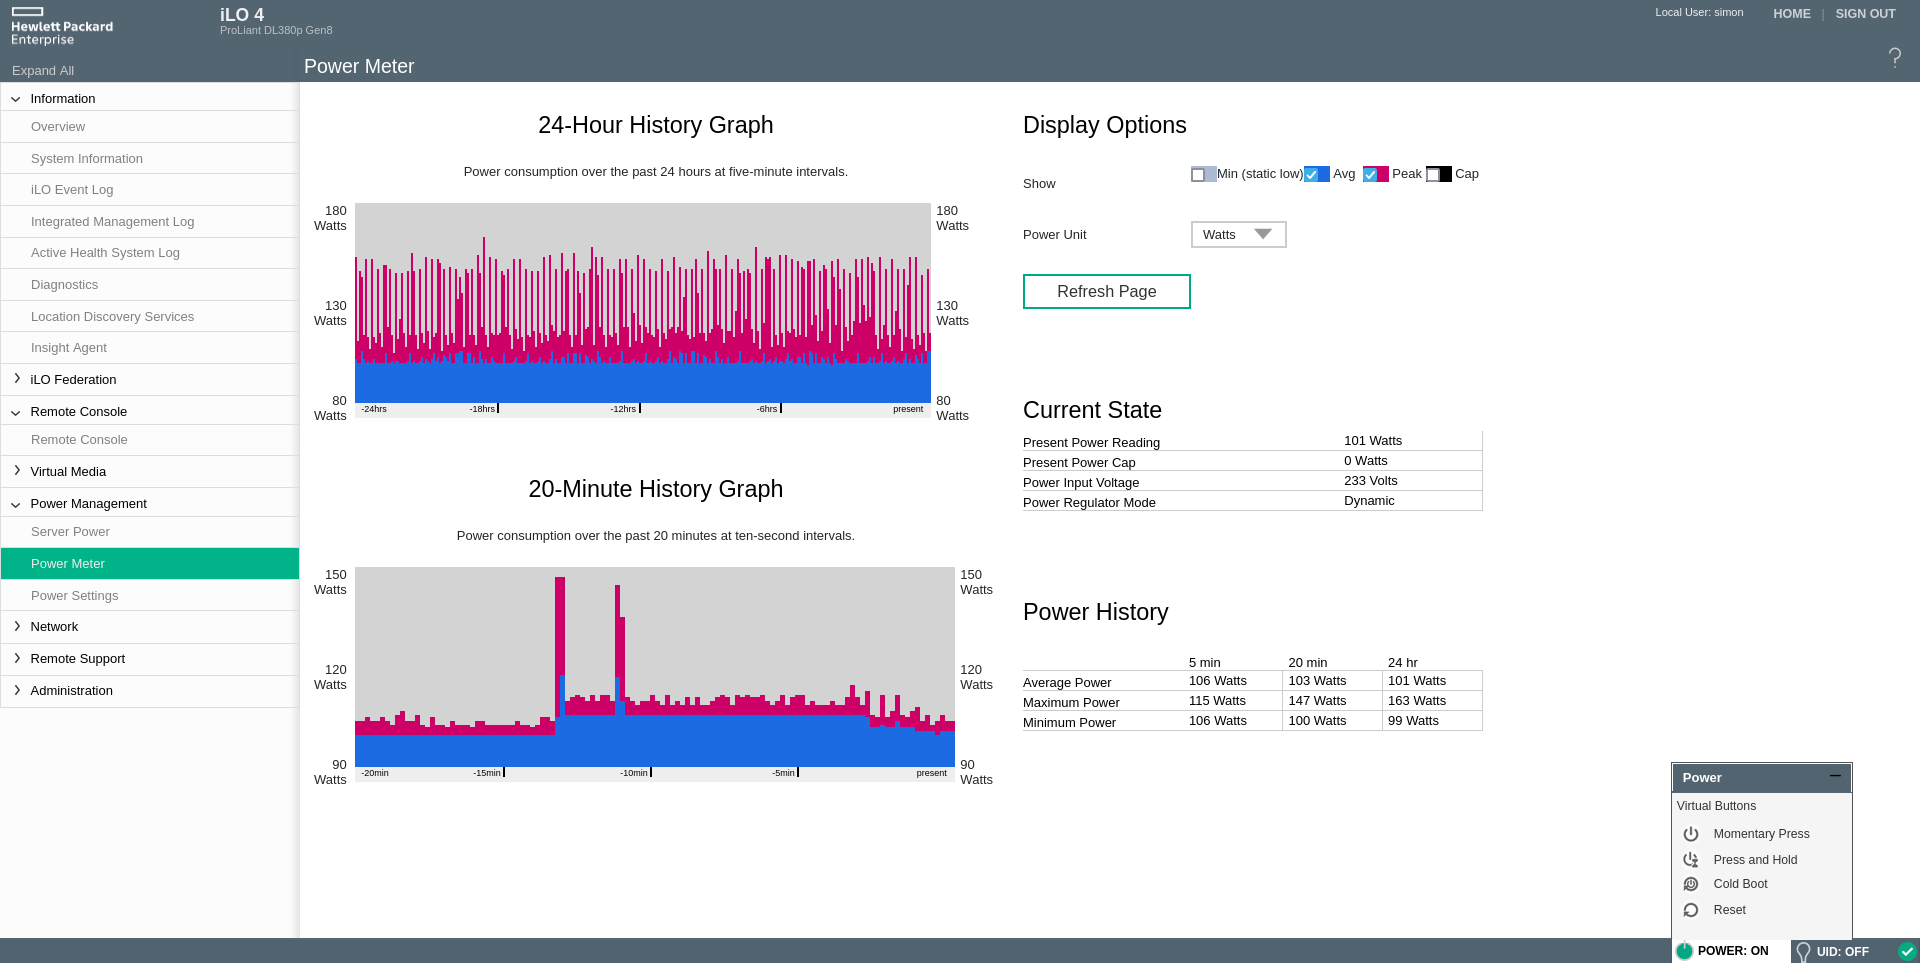
\includegraphics[width=150mm, keepaspectratio]{figures/ilo-power1.png}
	\caption{Szervergép fogyasztásának grafikonja egy HPE számítógép távoli menedzsment felületén. Vegyük észre a jobb alsó sarokban megjelenő menüt, amivel lehetőségünk van a gép kikapcsolására és újraindítására is.}
	\label{fig:ilopowerchart}
\end{figure}

A fent ismertetett üzemeltetést, karbantartást könnyítő felépítés mellett általában elmondható, hogy az ilyen gépek jelentős része virtualizációra van tervezve -- persze ezektől különböző felhasználási módok is jelentkeznek (például fájlszerverek tervezése során a teljesítmény helyett a minél nagyobb tárkapacitásra és adatátvitelre helyezték a hangsúlyt). A dolgozat szempontjából viszont a nagyvállalati környezetben domináló virtualizációs felhasználási terület lesz a lényegesebb, így a továbbiakban az ilyen számítógépekre fogok koncentrálni.

A virtualizációs hosztgépek jellemzője, hogy számos processzorral rendelkeznek, valamint felhasználói szemmel szokatlanul nagy memóriaterülettel bírnak. Ki fog derülni azonban, hogy 12-24 processzormag és akár több száz gigabyte RAM is szűkös erőforrássá válhat egy virtuális gépeket futtató számítógép esetében, hiszen gyakorlatilag itt egyetlen szervernek kell elbírnia akár több tíz számítógép terhelésével is. Ezek mellett általában több (8-24) háttértár-foglalattal is rendelkeznek, melyekhez hardveres RAID-támogatást is adnak.
% TODO: kép a gépről

\section{Virtualizáció}
\subsection{Áttekintés}
A virtualizáció egy olyan technológia, amely lehetővé teszi, hogy egy fizikai számítógépen (az úgynevezett virtuális host-on) több, akár a hosztgép rendszerétől eltérő operációs rendszert futtassunk. Ehhez szükség van egy \gls{hypervisor}-ra, ami az operációs rendszer legfőbb virtualizációt támogató komponense~\cite{Sles15virt}. Ez a szoftver közvetlenül a szerver hardverén fut, és ez biztosítja a virtuális gépek számára szükséges hardveres erőforrásokat virtualizált hardverinterfészeken keresztül. Szintén a \gls{hypervisor} felelős az erőforrások kezeléséért, tehát ennek a komponensnek kell biztosítania a virtuális gép számára beállított mennyiségű memória, processzor és háttértár rendelkezésre állását is. Ezek a beállítások a legtöbb modern \gls{hypervisor} esetében elvégezhetőek grafikus felületen is, erre ad példát \aref{fig:vboxsettings} ábra.

Napjainkban a legelterjedtebb hypervisorok közé tartozik a vmWare ESXi, a XEN és a KVM, melyek részletesebb bemutatását \aref{sect:hypervisor-comparision} alfejezet tartalmazza.

\begin{figure}[!ht]
	\centering
	\includegraphics[width=120mm, keepaspectratio]{figures/virtalbox-vm-settintgs.png}
	\caption{Virtuális gép beállításainak részlete a VirtualBox virtualizációs szoftverben.}
	\label{fig:vboxsettings}
\end{figure}


A virtualizáció számos előnnyel járhat az infrastruktúra és a kiszolgálni kívánt alkalmazások szempontjából. Az egyik legnagyobb ilyen előny például, hogy a virtuális gépek egymástól izoláltan futnak, azaz nincs közvetlen kapcsolat közöttük, ami biztonsági és kezelési, tesztelési szempontból (pl. egy adott csomag vagy szoftver kipróbálásához készíthetünk egy teszt virtuális gépet, amit egyszerűen törölhetünk a teszt végeztével; a telepített program eltávolítása hagyományos környezetben futtatva sokkal körülményesebb lenne) is kedvező lehet. Hasonlóan előnyökkel jár, hogy a legtöbb modern \gls{hypervisor} lehetőséget biztosít bizonyos erőforrások úgynevezett \gls{hotswap}-pelésére. Ez azt jelenti, hogy egyes komponenseket (pl. memória) úgy is bővíthetünk, hogy a rendszert nem szükséges ehhez leállítanunk.

\subsection{Paravirtualizáció és teljes virtualizáció}

\subsection{Virtualizációs lehetőségek összehasonlítása} \label{sect:hypervisor-comparision}

\section{Logikai kötetkezelés}
Mind a fizikai, mind a virtuális gépek esetén szükség lehet háttértárakra az adatok perzisztens tárolása érdekében. Hagyományos particionálási megoldásokkal hamar nehezen kezelhetővé válhatnak a különböző csatolási pontok és a virtuális gépek számára kiosztott kötetek. Az ilyen problémák elkerülésére jött létre a logikai kötetkezelés, mely a tárhely-virtualizáció egy formája. A logikai kötetkezelésnek több implementációja létezik. % TODO: cite wikipedia: https://en.wikipedia.org/wiki/Logical_volume_management
Ezek közül jelenleg a Linux kernelben elérhető \gls{lvm}-et fogom részletesen ismertetni.

A Linux logikai kötetkezelője három lényegi rétegből áll: a fizikai kötetből (physical volume, PV), a kötetcsoportból (volume group, VG) és a logikai kötetekből (logical volume, LV). Ezt a felépítést \aref{fig:lvm} ábra szemlélteti egy egyszerű \gls{lvm}-konfiguráción keresztül.
Lehetőség van ennél összetettebb kötetkiosztás létrehozására is, például egy kötetcsoport több fizikai kötetből is állhat, amik akár külön háttértáron is lehetnek, sőt, RAID-csoportot is megadhatunk egy \gls{lvm}-partíció alapjául. Ezen megoldások használata azonban sok hátránnyal járhat (pl. diszkhiba esetén nehezebb visszaállítani a partíciót), ezért ennek használata alapvetően nem ajánlott~\cite{RHLVM}.

Az \gls{lvm} tehát úgy épül fel, hogy egy vagy több háttértáron létrehozunk hagyományos fizikai partíciókat, melyek az \gls{lvm} \acrshort{pv}-k alapjául fognak szolgálni. Ezt követően létrehozzuk a kötetcsoportokat az általuk használandó \acrshort{lvm} fizikai kötetek megadásával. Az így létrejött csoportban már tudunk létrehozni logikai köteteket, amíg van szabad hely a \acrshort{vg}-ben.

Láthatjuk, hogy az \acrshort{lvm}-kötetek használata kezdetben több feladattal jár, mint a hagyományos partíciók esetében, azonban hosszabb távon számos előnnyel jár. Talán a logikai kötetkezelés legnagyobb előnye, hogy szabadon allokálhatunk tárterületet a létrehozott köteteknek: ha azt tapasztaljuk, hogy az egyik köteten kevés a szabad hely, akkor fájlrendszertől függően elég lehet akár egy parancs kiadása is ennek kiterjesztéséhez. Lényeges, hogy a hagyományos partíciók használatával ellentétben a logikai kötetkezelés használatakor figyelmen kívül hagyhatjuk a partíciók elhelyezkedésének sorrendjét, így nem szükséges figyelembe vennünk, hogy az adott partíció előtt vagy után van-e szabad tárterület. A megnövelt kötet helyes fizikai háttértárra képzéséről a logikai kötetkezelő fog gondoskodni számunkra. Fontos megjegyezni, hogy a kötetbővítés online is elvégezhető, azaz nem szükséges a kötetet lecsatolni a gépről az átméretezéshez. Ez különösen fontos lehet például a root~(/) partíció növelése során, hiszen ezt csak a számítógép leállítása mellett tudjuk biztonságosan lecsatolni. Előállhat olyan helyzet is, hogy egy másik (nem root) partíciót kell online átméreteznünk, például ha azt tapasztaljuk, hogy egy adatbázisszerveren hirtelen nagy mértékben nőtt a tárolt adat mérete. Ilyenkor nincs lehetőség a szerver leállítására, hiszen ez esetben az alkalmazások nem tudnák használni az adatbázist a leállás idejére. Az ehhez hasonló helyzetekre is jó megoldást nyújt a logikai kötetkezelő egy megfelelő, online átméretezést támogató fájlrendszer (pl. XFS, Btrfs) használata mellett. Érdemes megjegyezni, hogy bár az \acrshort{lvm} és például a Btrfs-fájlrendszer nyújt támogatást a növelésen kívül a fájlrendszer méretének csökkentésére is, ez a művelet általában nem biztonságos, és adatvesztéshez vezethet. Emiatt érdemes eleinte csak kisebb tárterületet adni a köteteinknek, hiszen kiterjeszteni sokkal egyszerűbb őket, mint csökkenteni a méretüket. Ennek megkönnyítésére is ad lehetőséget az \acrshort{lvm}, megadhatjuk, hogy egy kötet egy bizonyos arányú tárhelyhasználat után automatikusan bővüljön, így elkerülve annak betelését.

Az \acrshort{lvm} hasznos funkciói közé tartozik még a kötetpillanatképek (volume snapshots) készítésének lehetősége. Ez azt jelenti, hogy a kötetkezelő képes az adott kötet adott pillanatbeli helyzetének rögzítésére, és erre a verzióra szükség szerint visszaállhatunk (rollback). Ez hasznos lehet például nagyobb konfigurációs változások eszközölése esetén, gyorsan változó adatokkal dolgozó rendszerek (pl. adatbázisszerver) biztonsági mentéseinek készítése során, illetve rendszerfrissítések előtt.\footnote{Egyes eszközök és operációs rendszerek (pl. openSUSE-verziók a snapper-rel (\url{https://doc.opensuse.org/documentation/leap/reference/html/book-reference/cha-snapper.html}) automatikusan készítenek snapshotot a frissítések telepítése előtt, így hiba esetén visszaállhatunk a frissítés előtti verzióra.}



\begin{figure}[!ht]
	\centering
	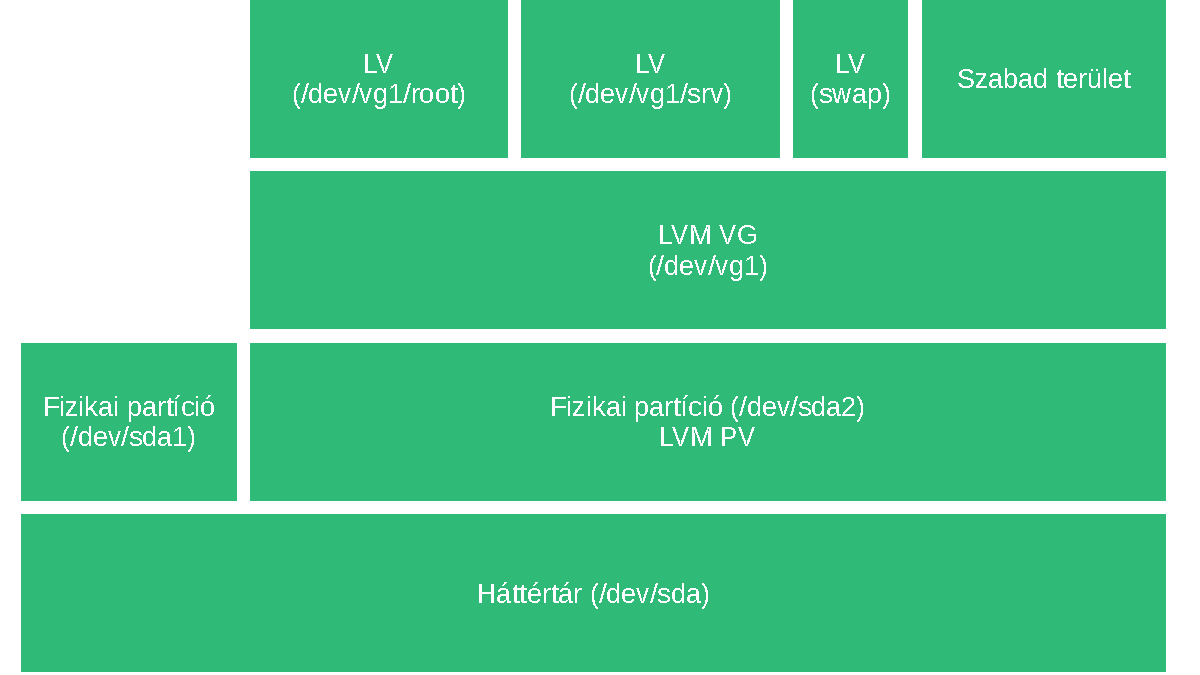
\includegraphics[width=14cm]{figures/lvm.pdf}
	\caption{Virtuális gép beállításainak részlete a VirtualBox virtualizációs szoftverben.}
	\label{fig:lvm}
\end{figure}

\section{OS-lehetőségek}
Debian/Ubuntu, RedHat, SuSE

\section{Eszközmenedzsment}

\section{Monitoring}